\chapter{Development}

This chapter describes the work methodology and the process used during this project. We compare two agile models and describe how we implemented scrum in our group. We also review some of the sprints, by looking at the results of the sprint as well as a retrospective look.

\section{Plan}

\subsection{Development Methodology}
The choice of methodology was mainly based on these three facts: The group has little experience with game engines, the group has little to no experience on working on a project of this scale and one of the requirements of \Gls{lokforerskolen} was that they would be tightly connected to the development and emphasized this connection in their task description.

Based on the three criteria stated above, the group concluded on using an agile software development model because it allows for rapid change in these requirements. It also allows for changes in the project scope without necessarily having major impacts on releases and planned progress.

\subsection{Development model}
When choosing the optimal model for our project we looked at several different models to see if they would fit our project. Two of the development models that got evaluated was \textit{\Gls{scrum}} and \textit{\Gls{kanban}}.

\Gls{scrum} is an agile development model. It is designed for teams of ten or fewer members who divide their work into increments of work within iterations called \gls{sprint}s, which are usually between two to four weeks long.\cite{atlassian_scrum_vs_kanban} Development teams utilizing \gls{scrum} meets once a day for 15 minutes or less to assess their progress and keep everyone up to date. There are also two other meetings that are important when working with \gls{scrum}; the \gls{sprint} review, which is often held together with the project stakeholder for feedback, and a retrospective meeting to reflect on the previous \gls{sprint} results.

\Gls{kanban} is also an agile development model, which visualizes the items or tasks from start to finish, usually through a \Gls{kanban} board.\cite{kanban_2022}. The main focus for teams working with \Gls{kanban} is reducing the time a project takes from start to finish by continuously improving their workflow.

The model we chose as our development model was \Gls{scrum}. The main reason for this was that although both methodologies could be utilized and work in our project, we wanted the main focus to be creating the best simulator as possible. \Gls{scrum}, in it's nature, allows and emphasises reflection and assessment every step of the way, and has a pre-decided structure for doing so. Scrum is also the development model which is most known and used by the group previously.  

\subsection{Our implementation of \Gls{scrum}}
We aimed to use the iterative nature of \Gls{scrum} to ensure the quality of the implementation at every stage of the project, and quickly adapt to any change in the client's specifications. In the beginning of the project we had one week \gls{sprint}s and continuously discussed if we needed to increase the \gls{sprint} duration, based on the upcoming tasks. We sought out to implement \Gls{scrum} in a strict way, with daily \Gls{scrum}-meetings throughout the project.

These meetings were used as a collaborative tool to identify problems if someone was stuck, keep everyone up to speed on the project process, and create a nice work environment where we kept in touch. We believe the latter was more important than it may have seemed, because most of the work is done from home, so it was nice to keep in touch with the group at least once every day. Although these meetings are important for the group, they could occasionally be skipped if they were unnecessary. 

For managing the project, we utilized \textit{Jira} integrated with \textit{GitHub}. This integration contributed to ensuring the methodology professionalism we aimed for in the project. We used constrained and secure workflows to ensure that every issue followed the correct workflow. In simpler terms, this set the rules for how all work was to be handled throughout the project. \ref{fig:workflow} shows the direction and constraints on how an issue can progress through the different statuses.

\begin{figure}[H]
\centerline{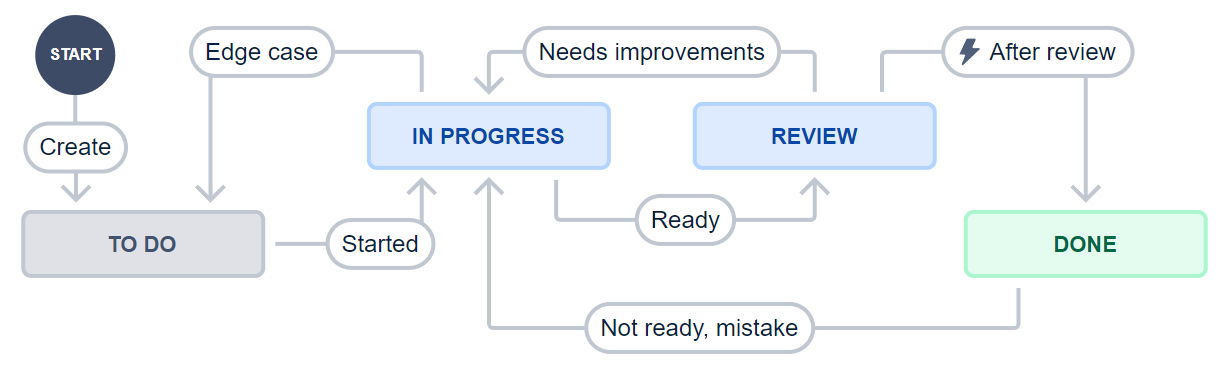
\includegraphics[width=1.0\textwidth]{figures/workflow.png}}
\caption{Issue status diagram}
\label{fig:workflow}
\end{figure} 

\subsection{Process Documentation}
\label{subsubsec:processdoc}

To log the time spent on the project, we planned to use \textit{Clockify} add-on for Jira. The add-on would allow the group to manually start a timer from within the issue in \Gls{jira}, tracking all work time until stopped. The elapsed time was manually logged along with a short comment of what was done that day. For planning the holistic overview of the project, we planned to use BigGantt. This is an extension to Jira which allows us to create a Gantt-chart in the same environment as our issues. 

\subsection{Code Documentation}

To ensure the quality and professionalism of the project we searched for and agreed upon some code conventions for \cpp programming in Unreal Engine, and standards for development. These conventions can be found in the appendix \ref{CodeConvention}. This document introduces \textit{Doxygen}, a documentation generator we utilized for automatically producing code documentation for the client. We saw this as a necessity, especially because we were writing code for a client. To do this, we had to follow Doxygen's documentation standard when commenting code. When the development came to a conclusion, we generated a folder of HTML-files, which can be hosted as a website to display the documentation. It is located inside the \verb|/Documentation|-folder in the project repository. 


\begin{figure}[H]
\centerline{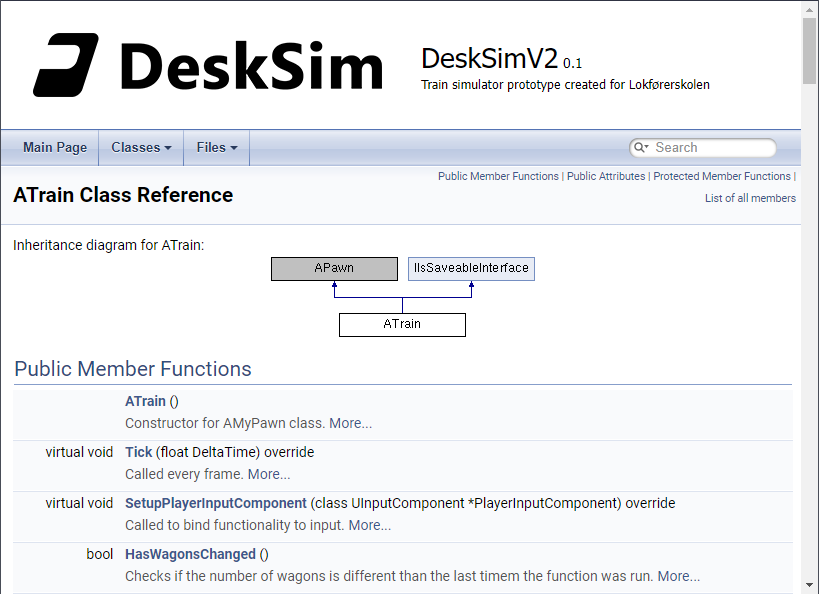
\includegraphics[width=1.0\textwidth]{figures/Documentation1.png}}
\caption{The documentation page for the ATrain class}
\label{fig:Documentation1}
\end{figure} 

The documentation contains all files, classes, functions and variables used in the project, and presents the user with menus, lists and a search bar for easy navigation. As shown in \ref{Documentation1}, a class page displays all relevant information for a class. Figure \ref{Documentation2} is captured further down on the same page, showing an example for a member function description. 

\begin{figure}[H]
\centerline{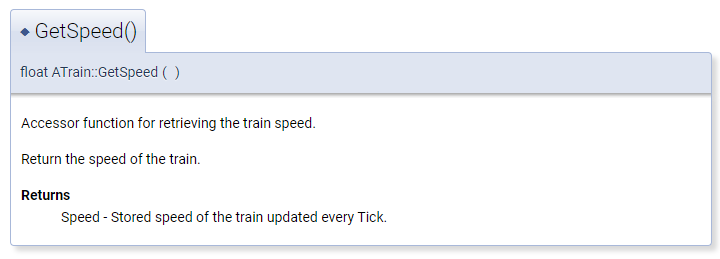
\includegraphics[width=1.0\textwidth]{figures/Documentation2.png}}
\caption{The documentation for ATrain member function GetSpeed}
\label{Documentation2}
\end{figure} 

\subsection{Git Workflow}
The group agreed upon some rules for working with git. these rules were made to ensure that the code was well protected against human error. The workflow consists of seven rules and it is mandatory for all group members to follow.

\begin{itemize}
\item Always create a new branch when starting work on a feature. No work should be done directly on the main branch.
\item This is, and should be the naming convention for branches: \\
\verb|<issue_number>-<branch_name>|
\item This is, and should be the only commit convention: \\
\verb|[#<issue-number>]-<description>|
\item When the work is completed on a branch, it must be deleted after the work is merged into the main branch.
\item Code should be committed often, either when a task is finished or the newly written code is fully functional.
\item Do not commit code that doesn't compile. Code should be tested before it is committed.
\item When a feature is complete, its branch should be merged into the current milestone branch. When the work for one milestone is completed, this branch should be merged with main. % Your own branch?



\end{itemize} 

\todo{config?? hmm. kopier noe fra prosjektplanen om git workflow}


\subsection{Gantt Chart}

Figure \ref{gannt_chart} presents the milestones for the project and their planned time schedule. This chart is a visualization of the planned project process, and it will be compared to the actual project process in \ref{deviation_process}. % Kanskje linke til en større versjon i appendices?

\begin{figure}[H]
\centerline{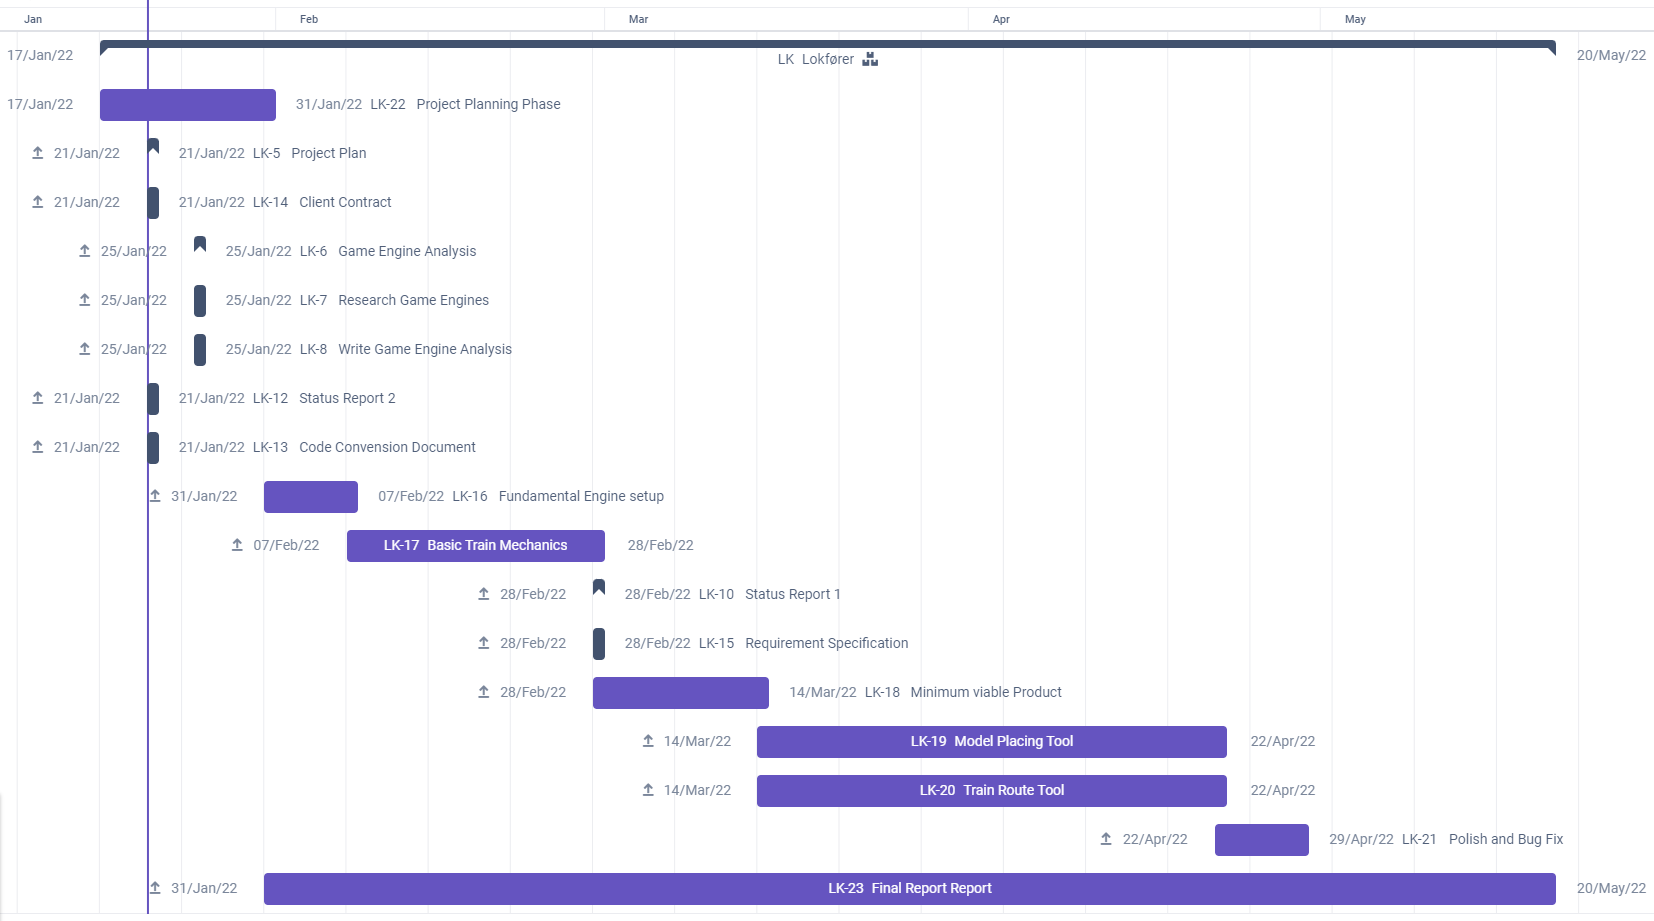
\includegraphics[width=1.0\textwidth]{figures/Gantt.png}}
\caption{Gantt chart}
\label{gannt_chart}
\end{figure} 



\begin{comment}
This chapter will provide a detailed description the methodology, and how we used it. It will describe some of our sprints and the project process as an entirety. There will also be a graphical view of the sprints showing the progress, and explanations over changes in the project scope.
\end{comment}



\section{Process}

This section will describe our usage of development tools such as \Gls{jira}. It will also cover the estimation process, examples of weekly \glspl{sprint} and a overview over the changes and deviation from the original project plan.

\subsection{\Gls{jira}}

The group used \Gls{jira} for implementing scrum into our project. We created our product backlog and kept track over all issues and \glspl{sprint} in the software. To use Jira to the full extent we had to follow the git workflow. When a push was made to GitHub, using the correct commit conventions provided a commit history available in the software. 

\begin{figure}[H]
\centerline{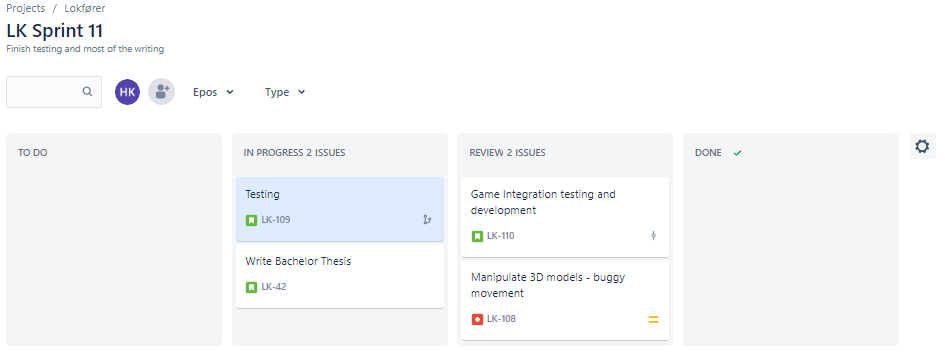
\includegraphics[width=1.0\textwidth]{figures/Jira_scrum board.PNG}}
\caption{Scrum board in Jira Software}
\label{gannt_chart}
\end{figure} 


\subsection{Sprints}
Our project consisted of eleven sprints. Figure \ref{sprint_overview_img}, contains a visualization of the main focus area for each of the sprints. Sprint three, seven and eleven is displayed below to give an example of how the group approached and solved issues related to setting up, developing and testing the system. For each of the sprint's a table is displayed to show the result of the sprint with the estimations made.


\begin{figure}[H]
    \centering
    \vspace{12pt}
    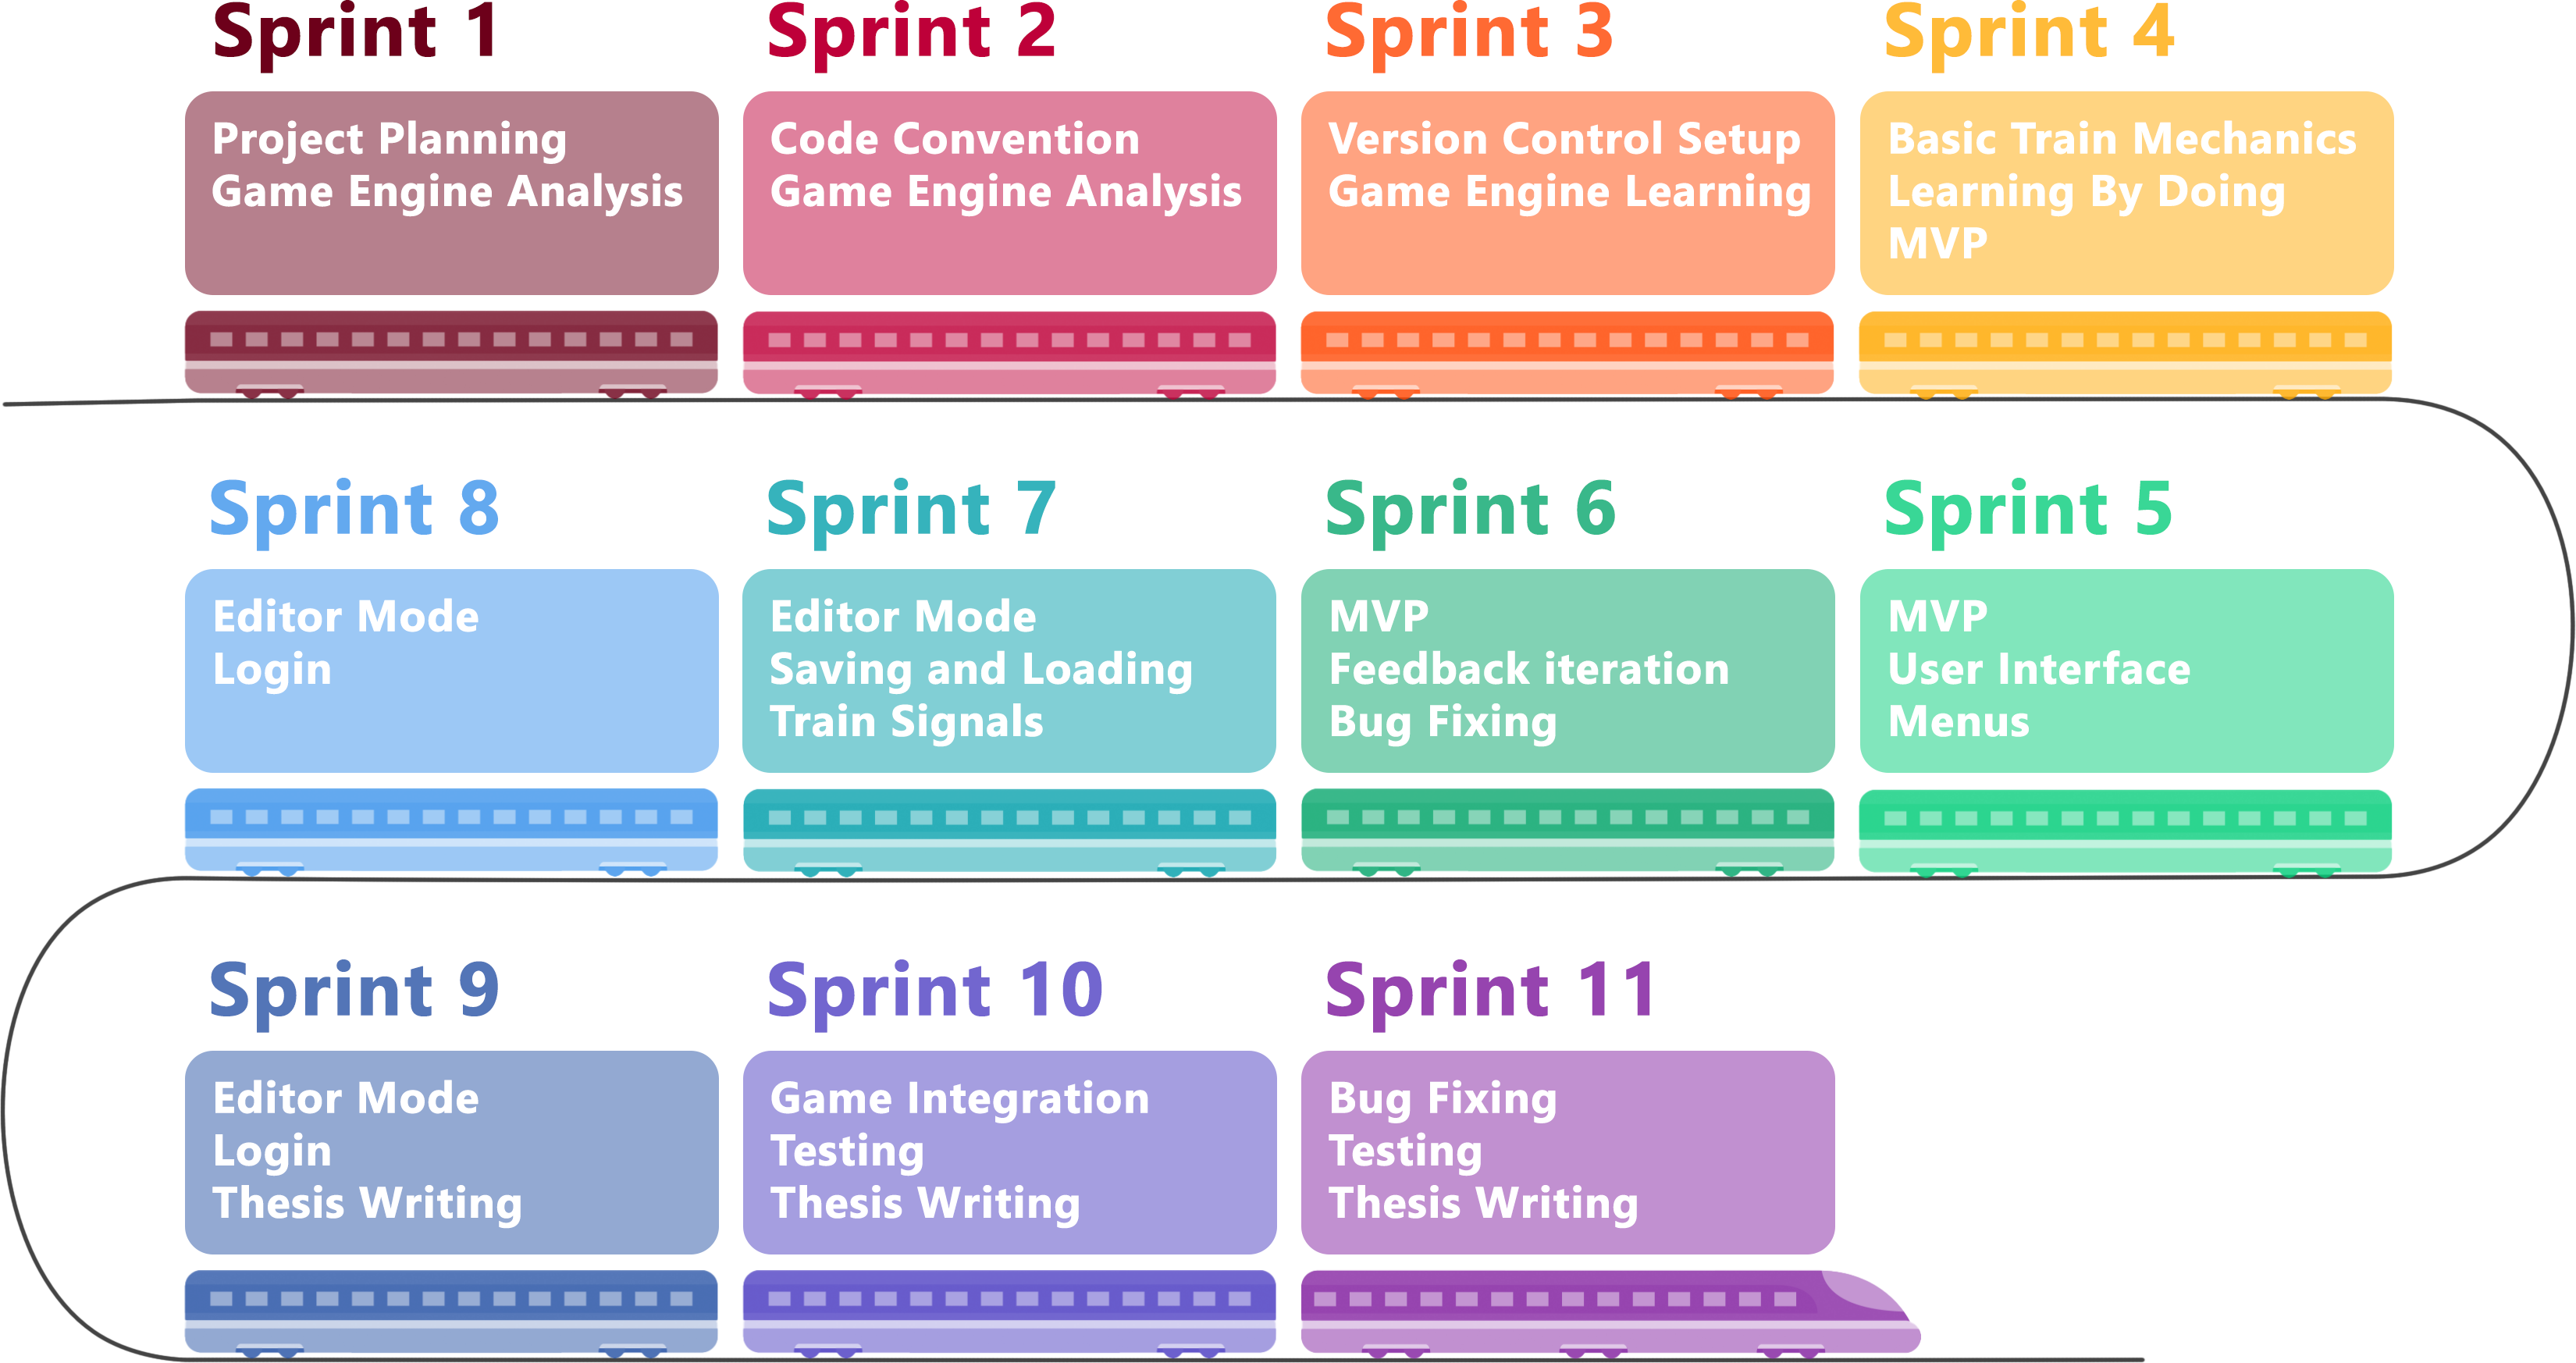
\includegraphics[width=\textwidth]{figures/SprintModel.png}
    %\vspace{-12pt}
    \caption{Overview of all sprints}
    \label{sprint_overview_img}
\end{figure} 

The sprint meeting notes are written with three different sections. A section about the Goals we have for the sprint. A section which discusses the result of the sprint. And a retrospective section where we will discuss and reflect on the result of the sprint with the goals in mind. 

\textbf{Estimations} \\
We started out estimating issues in T-shirt sizes, ranging from 1-4 which imitates small, medium, large and extra large issues. After sprint 3 we decided to change the estimation strategy to hopefully estimate more accurately. We changed the estimations to be an exact number, but tried to keep the task sizes low.

\textbf{Statuses} \\
The issues can be set to one of five statuses describing its current state in a sprint. The statuses are: \\
\textbf{Wishlist} - The issues that is taken out of the project scope and in to a list of functionality that we can decide to include if we have time later in the project. \\
\textbf{To Do} - This are the section for issues that are waiting to be developed. \\
\textbf{In Progress} - The issues that are currently being developed.
\textbf{Review} - The issues that is currently under review by peers.
\\
\textbf{Done} - The issues that has been completed in the sprint.\\

\begin{large}
    \textbf{Sprint 3} \\
\end{large}
\textbf{Date:} 07.02.2022 \\ 
\textbf{Present:} Endre, Henrik, John Ole and Thomas \\
\textbf{Period:} 07.02 - 14.02 \\ 

\textbf{Sprint Goal:}
\begin{itemize}
    \item Review and deliver Game Engine Analysis to the client and to our supervisor
    \item Integrate Jira with GitHub
    \item Setup the repository in GitHub with an Unreal project
\end{itemize}

\textbf{Sprint result:} \\
“This is the first sprint where we managed to get all our goals finished in time. We managed to finish the setup and integration with Jira on time, which resulted in being able finish the MVP within two weeks.”

%This is the first sprint that we actually managed to get all our goals finished in
%time. We managed to finish the setup and integration with Jira and this results
%in a decrease of time delay from our original plan to be finished with the MVP in
%two week
%a decrease of time delay from our original plan to be finished with the MVP within two weeks. \todo{siste setningen her ??}

\begin{table}[H]
    \centering
    \begin{tblr}{
      colspec={|X[0.20, l]|X[0.30, l]|X[0.50, l]|}, hlines,
      column{1} = {gray9},
      column{2} = {purple9},,
      column{3} = {green9},
      row{2} = {c}
    }
    \SetCell{bg=gray4}  & \textbf{Other statuses} & \textbf{Done} \\
        Issues & - & \SetCell[c=1]{l}  Write Engine Analysis \newline\newline Integrate GitHub and Jira \newline\newline Setup Repository \newline\newline Code Convension Document \newline\newline Learning Engine Basics \\
        Estimates & \SetCell[c=1]{c} 0 & \SetCell[c=1]{c} 4 + 2 + 2 + 2 + 2
    \end{tblr}
     \caption{Overview of issue status at the end of sprint 3}
\end{table}

\textbf{Retrospective:} \\
“We finished all the tasks we had in mind and also managed to start learning the engine basics as well. This means that we from next week can start working towards the MVP. We discussed increasing the sprint length from one to two weeks for the next sprint, but decided to keep the one week sprint because we want to have a new retrospective meeting next week and evaluate the accuracy of the story point estimates we made on the issues regarding the MVP to figure out if we can finish the MVP in the allocated time. This decision was made because the time we have set to be finished with the MVP and display it to the client is the 14th of March.”


\begin{large}
    \textbf{Sprint 7} \\
\end{large}
\textbf{Date:} 07.03.2022 \\ 
\textbf{Present:} Endre, Henrik, John Ole and Thomas \\
\textbf{Period:} 07.03 - 21.03 \\ 

\textbf{Sprint Goal:}
\begin{itemize}
    \item Finish first draft of requirement specification and status report 1.
    \item Finish the MVP scenario
\end{itemize}

\textbf{Sprint result:} \\
“The MVP got finished and put together. We had some issues with the environment creation and it's time consumption, but the estimations we made for three environment creation tasks was more accurate than our previous estimations. All the necessary functionality was there to display the MVP to the client except the basic statuses which we only controlled by a timer instead of an controller. The basic statuses was only missing a few hours of work and is therefore almost finished.”

\begin{table}[H]
    \centering
    \begin{tblr}{
      colspec={|X[0.15, c]|X[0.21, c]|X[0.21, c]|X[0.21, c]|X[0.22, c]|}, hlines,
      column{1} = {gray9},
      column{2} = {purple9},
      column{3} = {blue9},
      column{4} = {blue9},
      column{5} = {green9},
    }
    \SetCell{bg=gray4}  &
    \textbf{Wishlist} &
    \textbf{To do} &
    \textbf{In Progress} &
    \textbf{Done} \\
        Issues 
        & \SetCell[c=1]{l} Editor mode: \newline - Generate flat terrain (14) \newline - Manipulate terrain (20) \newline - Dynamic buttons (10)
        & \SetCell[c=1]{l} Place and edit railway (28) \newline \newline Load scenario from file (14) \newline \newline Save scenario to file (14) Static Buttons on screen (7)
        & \SetCell[c=1]{l} Main Goal: \newline - Signal Controller (21) \newline - Emergency Breaks (7) \newline - Stop Scenario (21) \newline \newline In game content browser (25) \newline \newline Save Object to File (20) \newline \newline Load Object From File (20)
        & \SetCell[c=1]{l} Main Menu (14) \newline \newline Basic Statuses (7) \newline \newline Second iteration Requirement Specification (21)  \newline \newline Place 3D Models (12) \newline \newline Manipulate 3D Models (25)  \\
        Estimates & 44 & 63 & 114 & 79
    \end{tblr}
     \caption{Overview of issue status at the end of sprint 7}
\end{table}


\textbf{Retrospective:} \\
“The sprint goals was achieved, but the basic statuses was only implemented to work with the MVP scenario and not finished to he extent we want in the final product. We want the signals to be controlled by a controller and be able to trigger events. New issues for this will come in the next sprint. We finished 93 work hours in the sprint and we feel that our estimations on the different tasks are beginning to get better and more accurate to how we progress in the sprints.”

\begin{large}
    \textbf{Sprint 10} \\
\end{large}
\textbf{Date:} 21.02.2022 \\ 
\textbf{Present:} Endre, Henrik, John Ole and Thomas \\
\textbf{Period:} 18.04 - 01.05 \\ 

\textbf{Sprint Goal:}
\begin{itemize}
    \item Finish the demo test level
    \item Have the simulator ready for testing (all functionality ready)
\end{itemize}

\textbf{Sprint result:} \\
“We finished the demo test level and got the simulator ready for the student tests. The process was challenging because it was important that the quality was ensured because the simulator is going to be tested on students from Lokførerskolen next Monday.”

\begin{table}[H]
    \centering
    \begin{tblr}{
      colspec={|X[0.15, c]|X[0.28, c]|X[0.28, c]|X[0.29, c]|}, hlines,
      column{1} = {gray9},
      column{2} = {purple9},
      column{3} = {blue9},
      column{4} = {green9},
    }
    \SetCell{bg=gray4}  &
    \textbf{Wishlist} &
    \textbf{In Progress} &
    \textbf{Done} \\
        Issues 
        & \SetCell[c=1]{l} Place and Edit Railways (28) 
        & \SetCell[c=1]{l} Write bachelor Thesis (30) \newline \newline Game integration testing (30)
        & \SetCell[c=1]{l} Basic Train cars (10) \newline \newline Convert in-game menu to c++ (4) \newline \newline Demo Test Level: \newline - Create Environment (4) \newline - Add train and wagon (1) \newline Add signal and triggerboxes (2) \newline - Add railway (2) \newline - Add station (1) \newline - Possesion switch between drone and train (2) \newline Fix camera possesion bug (4) \newline \newline Delete editor objects (5) \\
        Estimates & 28 & 60 & 21
    \end{tblr}
     \caption{Overview of issue status at the end of sprint 8}
\end{table}


\textbf{Retrospective:}

“Even though we only finished 21 of the story point estimates, we have spent much time on writing the final thesis. All tasks we set out to do is finished except the Place and edit railway issue which got excluded from the project scope. This particular task was taking up a lot of development time due to the unforeseen difficulty of the task. After discussing internally and with the client, we concluded that all the functionality we were developing in the in-game editor mode were reflections of what offers in-engine. This made a hindrance to further development of editor functionality, which was then removed from the project, as the client agreed that it would be easier to utilize Unreal Engine itself for this functionality.

When planning the sprint we added an issue for game integration testing. This issue would contain all the bugs, errors and code mistakes we could find when trying to build and package the game. Since the scope of the issue increases when working on it, we decided to not include as much issues to this sprint to ensure that this issue gets the attention it needs.”

%%%%%%%%%%%%%%%%%%%%%%%%%%%%%%%%%%%% SCRUM %%%%%%%%%%%%%%%%%%%%%%%%%%%%%%%%%%%%%%%%%%

\subsection{Deviation from original plan} \label{deviation_process}
While developing the simulator we encountered some situations where we decided to or were forced to deviate from our original plan. This section will explain the main deviations, and they will be addressed further in the discussion \todo{reference discussion}  

\subsubsection{Deviations in project process plan}
Figure \ref{Epic_comparison_img} shows the milestones for the project with it's allocated time period. There were some deviations in the project process compared to what we planned in the beginning of the project. As the figure shows our planned progress was fairly similar to the planned process, but it was some delays in the beginning of the project. some milestones was being worked on in the same time such as basic train mechanics and minimum viable project. There was also a new milestone (Testing and Game Integration) we did not expect was going to take up as much time as it did.

\subsubsection{Deviation in estimation process}

As previously stated the estimations was done in T-Shirt sized estimations. We did not find these estimations valuable when working with scrum. Further estimations did not get easier after reviewing the T-shirt sized issues because it had margins such as 1-3 hours, 1 day and 2-3 days. We wanted to change it to get an exact value we could utilize to set better and more realistic estimations.

\begin{figure}[H]
    \centering
    \vspace{12pt}
    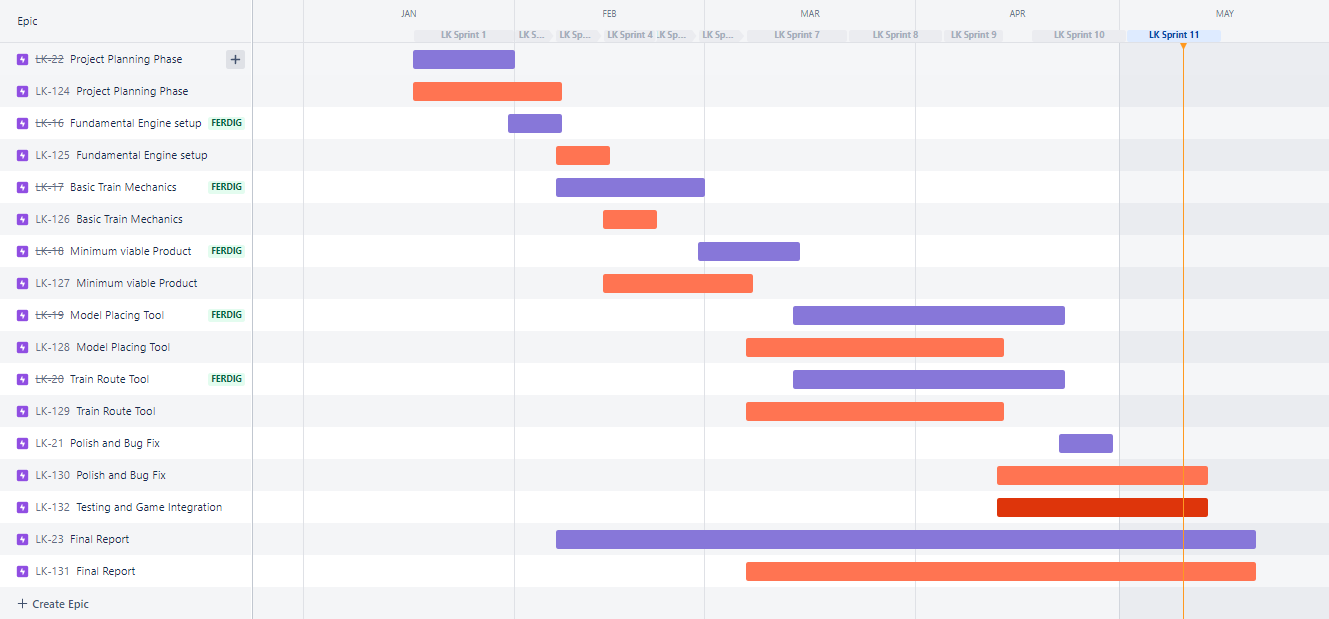
\includegraphics[width=12cm]{figures/Jira comparisoncroped.png}
    \caption{Comparison of original project plan (purple), to the actual project process (orange). The red bar shows an epic in the development we did not plan for but that was necessary to include}
    \label{Epic_comparison_img}
\end{figure} 

\subsubsection{Daily scrum meetings}

The daily scrum meeting worked well in the beginning of the project. We were all sharing our experiences and letting the group know what we had done the previous day and making sure everyone know the current status of the project. After one month of the development process these meeting began to feel forced and not very productive, they often went way over the time limit and noting them down just seemed like a waste of time. We therefore decided to stop doing these meeting as a forced, structural procedure. We did not stop having the meetings but we only noted them down when there was any relevant information that needed to be addressed later in the development which had not been addressed in the retrospective meetings.

\subsubsection{Sprint lengths}

We started the project with a sprint length of one week. After sprint 6 we decided to increase the length to two weeks because of the increase of magnitude in the upcoming milestones with was the model placing and train route tool. This decision was made as previously stated in the retrospective for week 6 to produce more functionality and give our self more time to produce code before evaluating it. The rapid time between development and planning also became more an obstacle than a benefit for us as it began to halt the process by only allowing us to finish small sections of the functionality at a time.

% Disse kan egt splittes opp, så ^denne er her, og vdenne er i discussion

The change in the sprint length also provided us with the opportunity to take a rest day or a research day. This day was allocated at the beginning of each sprint after sprint 7. This day was voluntary for each member of the group and the different group members used the day differently. Some used it to continue working on the previous sprint, some used it to write about the implementations they had done in the previous sprint, and some took an extra day of rest.
